\documentclass[../thesis.tex]{subfiles}

\begin{document}
\chapter{Mathematical Background}\label{ch:math-background}

A solid mathematical introduction is key to understanding how and why the approach
in this thesis works. This chapter serves as a primer to differential geometry and frame fields.
\section{Differential Geometry}
We will make heavy use of differential geometry in chapter \ref{ch:connection}.
I introduce the basic concepts what we will use, but I refrain from
giving any proofs. The following is an incomplete summary of concepts that we need presented in
\emph{Introduction to smooth manifolds}\cite{LeeManifold}.

\subsection{Manifold} A manifold $\mathcal{M}$ is a space that locally looks like Euclidean space.
More exactly, a $n$-manifold is a topological space, where each point on the manifold has an open neighborhood
that is locally homeomorphic to an open subset of Euclidean space $\mathbb{R}^n$.
A manifold can be equipped with additional structure. For example, we can work on \emph{smooth manifolds}.
In simple terms, a manifold is \emph{smooth} if it is similar enough to $\mathbb{R}^n$ that we can do Calculus
like differentiation or integration on it. For this, each point on the manifold must be
locally \emph{diffeomorphic} to an open subset of $\mathbb{R}^n$ space.
In this thesis, we will mostly work with 3-manifolds. For easier illustration, some examples are in 2 dimensions.

\subsection{Tangent space, Tangent bundle} There are many equivalent definitions
for the tangent space. The tangent space is a vector space which has the same dimension as its manifold,
which is 3 in our case.
One definition is for each point $p$ in the mani-fold $\mathcal{M}$,
the tangent space $T_p\mathcal{M}$ consists of $\gamma'(0)$ for all differentiable paths ${\gamma: (-\varepsilon, \varepsilon) \to \mathcal{M}, \varepsilon > 0}$
with $p = \gamma(0)$.
These tangent spaces can be ``glued'' together to form the
\emph{tangent bundle} $T\mathcal{M} = \sqcup _{p \in \mathcal{M}}T_p\mathcal{M}$, which itself
is a manifold of dimension $2n$. An element of $T\mathcal{M}$ can be written
as $(p,v)$ with $p \in \mathcal{M}$ and $v \in T_p\mathcal{M}$. This admits a natural projection $\pi : T\mathcal{M} \to \mathcal{M}$,
which sends each vector $v \in T_p\mathcal{M}$ to the point $p$ where it is tangent: $\pi(p,v)=p$.
A \emph{section} $\sigma: \mathcal{M} \to T\mathcal{M}$ is a continuous map, with $\pi \circ \sigma = \Id_{\mathcal{M}}$.
Sections of $T\mathcal{M}$ are tangent vector fields on $\mathcal{M}$.
An ordered $k$-tuple $(X_1, \dots, X_k)$ of vector fields is linearly independent,
if at each point $p$, the $k$-tuple $(X_1|_p, \dots, X_k|_p)$ is linearly independent.
A \emph{local frame for $\mathcal{M}$} is an ordered $n$-tuple of vector fields $(E_1, ..., E_n)$
defined on an open subset $U\subseteq \mathcal{M}$
that spans the tangent bundle $T\mathcal{M}$. Thus, $(E_1|_p,\dots, E_n|_p)$ form
a basis for $T_p\mathcal{M}$ for each point $p\in \mathcal{M}$.
A \emph{frame} is called \emph{smooth} if the underlying vector fields are smooth and \emph{global} if $U = \mathcal{M}$.

\subsection{Cotangent space, Cotangent bundle} The dual space $V^*$ of a vector space $V$
consists of all linear maps $\omega: V \to \mathbb{R}$. We call these functionals \emph{covectors} on $V$.
$V^*$ is itself a vector space, with the same dimension as $V$ and operations like addition and scalar multiplication
can be performed on its elements. Any element in a finite vector space can be expressed as 
a finite linear combination of its basis. The basis of a dual space is called the \emph{dual basis}.
Thus, we call the dual space of the vector space $T_p\mathcal{M}$ its \emph{cotangent space},
denoted by $T^*_p\mathcal{M}$. As before, the disjoint union of $T^*_p\mathcal{M}$ forms the \emph{cotangent bundle}:
$T^*\mathcal{M}=\sqcup _{p\in \mathcal{M}}T^*_p\mathcal{M}$. Defined analogously from above,
sections $\sigma$ on $T^*\mathcal{M}$ define \emph{covector fields} or \emph{1-forms}. The standard basis of $T_p^*\mathcal{M}$
is given by $\mathbb{E}^3=[dx,dy,dz]$.
A \emph{local coframe for $\mathcal{M}$} is an ordered $n$-tuple of covector fields
$(\mathcal{E}^1,\dots, \mathcal{E}^n)$ such that $(\mathcal{E}^i|_p)$ form a basis
of $T^*_p\mathcal{M}$ at each point $p \in \mathcal{M}$. This definition is analogous from
before.
For each local frame $(E_1, \dots, E_n)$ for $T\mathcal{M}$, we get a uniquely
determined local coframe $(\mathcal{E}^1, \dots, \mathcal{E}^n)$ such that
$\mathcal{E}^i(E_j)=\delta^i_j$, where $\delta^i_j$ is the Kronecker delta.
We call this coframe the \emph{dual coframe to $(E_i)$}.



\subsection{Tensors}
Before we can introduce differential forms in the next paragraph, we need to go a little bit into \emph{tensors}.
In simple words, tensors are real-valued, multilinear functions.
A map $F: V_1 \times \dots V_k \to W$ is multilinear, if $F$ is linear in each component.
For example, consider the \emph{Tensor Product of Covectors}:
Let $V$ be a vector space and take two covectors $\omega, \eta \in V^*$.
Define the new function $\omega \otimes \eta: V\times V \to \mathbb{R}$ by
$\omega \otimes \eta (v_1,v_2) = \omega(v_1)\eta(v_2)$. It is multilinear, because $\omega$ and $\eta$ are linear.

We look at a special class of tensors, the \emph{alternating tensors}.
A tensor is alternating, if it changes sign whenever two arguments are interchanged,
i.e. $\omega(v_1, v_2) = -\omega(v_2, v_1)$.
A covariant tensor field over a manifold defines a covariant tensor at each point on the manifold,
covariant because the tensor is over the cotangent space $T^*_p\mathcal{M}$.
An alternating tensor field is called a \emph{differential form}.

\subsection{Differential Forms, Exterior Derivative}
Recall that a section from $T^*\mathcal{M}$ is called a differential 1-form, or just 1-form.
We define the \emph{wedge product} (or \emph{exterior product}) between two 1-forms:
$$(\omega \wedge \eta)_p = \omega_p \wedge \eta_p$$
Notice the similarity to the \emph{Tensor Product of Covectors}: We get a new map, (a 2-form):
$$\omega \wedge \eta: T\mathcal{M} \times T\mathcal{M} \to \mathbb{R}$$
The wedge product is antisymmetric, therefore $\omega \wedge \eta = -\eta \wedge \omega$ for 1-forms $\omega$ and $\eta$.
We denote by $\Omega^k(\mathcal{M})$ the space of differential $k$-forms on $\mathcal{M}$.
There is a natural differential operator $d$ on differential forms we call \emph{exterior derivative}.
It maps $k$-forms to $(k+1)$-forms, i.e. $d: \Omega^k(\mathcal{M}) \to \Omega^{k+1}(\mathcal{M})$
and has the the following properties:
\begin{itemize}
  \item $df$ is the ordinary differential of a smooth function $f$. Smooth functions are 0-forms.
  \item $d(d\alpha) = 0$
  \item $d(\alpha \wedge \beta) = (d\alpha \wedge \beta) + (-1)^k(\alpha \wedge d\beta)$ for a $k$-form $\alpha$ (Leibnitz Rule).
\end{itemize}
In section \ref{ch:connection} we will need what $d\omega$ is for some smooth 1-form $\omega$, the calculation
will be done there. For now, just note that 
any smooth 1-form can be written as $\omega = Fdx+Gdy+Hdz$ for some appropriate smooth functions $F,G,H$
with the standard basis $\mathbb{E}^3$.


\subsection{Riemannian metric, $g$-orthonormality}
Inner products $\langle \cdot , \cdot \rangle$ are examples of symmetric tensors. They allow us to define lengths and angles
between vectors. We can apply this idea to manifolds.
A Riemannian metric $g$ is a symmetric positive-definite tensor field at each point.
If $\mathcal{M}$ is a manifold, the pair $(\mathcal{M},g)$ is called a \emph{Riemannian manifold}.
Let $g$ be the Riemannian metric on $\mathcal{M}$ and $p\in \mathcal{M}$,
then $g_p$ is an inner product on $T_p\mathcal{M}$. We write $\langle \cdot, \cdot\rangle_g$ to denote this inner product.
Any Riemannian metric can be written as positive-definite symmetric matrix $g$, which allows for this simple form: $\langle v,w\rangle_g = v^{\top}gw$.

Such a new metric allows for the definition of \emph{$g$-orthonormality}:
A basis $[e_1, e_2, e_3]$ of $T_p\mathcal{M}$ is $g$-orthonormal if $\langle e_i, e_j \rangle_g = \delta_{ij}$.

\subsection{Connection, Covariant derivative, Parallel transport}
A connection defines how two different tangent spaces are connected to each other, such that tangent vector fields
can be differentiated. There is an infinite amount of connections on a manifold.
An \emph{affine connection} $\nabla$ is a bilinear map that takes two tangent vector fields $X,Y \in \mathcal{T}(\mathcal{M})$ and maps it
to a new tangent vector field $\nabla_XY \in \mathcal{T}(\mathcal{M})$ such that
\begin{itemize}
  \item $\nabla_{fX}Y = f \nabla_XY$, where $f\in C^{\infty}(\mathcal{M}, \mathbb{R})$
  \item $\nabla_X(fY) = f\nabla_XY + (Xf)Y$ for $f\in C^{\infty}(\mathcal{M}, \mathbb{R})$, it satisfies the Leibnitz rule in the second variable
\end{itemize}
We call $\nabla_XY$ the \emph{covariant derivative of $Y$ in the direction of $X$}.
A connection $\nabla$ defines the parallel transport
of a vector along a curve. Given a curve $\gamma: [0,1] \to \mathcal{M}$ and
a vector $v_0 \in T_{\gamma(0)}\mathcal{M}$, there exists a unique parallel vector field $V: [0,1] \to T\mathcal{M}$ along $\gamma$
such that $V(0) = v_0$ \cite{LeeCurvature}.
Recall: a vector field $V$ along $\gamma$ means $\pi(V(t))=\gamma(t)$.
The uniqueness and existence is a consequence of the vector field $V$ being the solution
of $\nabla_{\dot{\gamma}(t)}V(t) = 0$ defining a linear ordinary differential equation with initial condition
$V(0)=v_0$. This vector field $V(t)$ is called the \emph{parallel transport} of $v_0$ along $\gamma$.
It is ``parallel'' in the sense that the transported vector does not change within the tangent space.
See figure \ref{fig:vectorfield} for an illustration in 2D.
\begin{figure}[htb]
  \centering
  \def\svgwidth{20em}
  \input{figures/vektorfeld.pdf_tex}
  \caption{A parallel vector field $V(t)$ along a curve $\gamma$. Each $V(t)\in T_{\gamma(t)}\mathcal{M}$ and
  $\nabla_{\dot{\gamma}(t)}V(t) = 0$, so each vector that is drawn is parallel to each other.}
  \label{fig:vectorfield}
\end{figure}

In the following, we show how a connection can be written as a matrix 1-form:
Let $(E_1, E_2, E_3)$ be a smooth local frame for $T\mathcal{M}$ and
$(\mathcal{E}^1, \mathcal{E}^2, \mathcal{E}^3)$ its dual coframe for
$T^*\mathcal{M}$ i.e. $\mathcal{E}^i(E_j)=\delta^i_j$.
Using the definition of an affine connection, we can write
vector fields $X,Y \in \mathcal{T}(\mathcal{M})$ with the local frames, i.e.
\begin{equation}\label{eq:rewrite}
  \nabla_XY = \nabla_{X^iE_i}(Y^iE_j) = X^i\nabla_{E_i}(Y^iE_j)
  = \underbrace{X^iY^j}_{\in C^{\infty}(\mathcal{M}, \mathbb{R})} \cdot \underbrace{\nabla_{E_i}E_j}_{\in \mathcal{T}(\mathcal{M})} + \underbrace{X^iE_i(Y^j)}_{\in C^{\infty}(\mathcal{M}, \mathbb{R})}\cdot \underbrace{E_j}_{\in \mathcal{T}(\mathcal{M})} \in \mathcal{T}(\mathcal{M})
\end{equation}
Because $\nabla_{E_i}E_j \in \mathcal{T}(\mathcal{M})$, we can also write this in the local frame $(E_1, E_2, E_3)$,
that is, for all pairs of indices $i,j \in \{1,2,3\}$, we write
$$\nabla_{E_i}E_j = \Gamma_{ij}^kE_k$$
The $\Gamma_{ij}^k$ are called \emph{Christoffel symbols} or \emph{connection coefficients}.
With these coefficients, we can rewrite equation \ref{eq:rewrite} to 
\begin{equation}
  \nabla_XY = X^iY^j \Gamma_{ij}^kE_k + X^iE_i(Y^j) E_j = X^i(X^iY^j\Gamma_{ij}^k + E_i(Y^k))E_k
\end{equation}
where the dummy index $j$ was renamed to $k$ in the last term (we are using Einstein summation convention, so the indices are independent).
This derivation shows that the choice of $\Gamma_{ij}^k$ fully determine the connection $\nabla$.
We can now define another connection $\Hat{\nabla}$ with 1-forms:
\begin{equation}
  \Hat{\nabla}_X (Y^jE_j) \triangleq X(Y^j)E_j + Y^j \Hat{\nabla}_X E_j \qquad \text{where } \Hat{\nabla}_XE_j = \omega_j^k(X)E_k
\end{equation}
and $\omega_j^k$ are 1-forms. It thus satisfies the Leibnitz rule in the second variable.
To show that it is indeed a connection, it must also satisfy $C^{\infty}$ linearity in the direction of $X$, i.e.
\begin{equation}
  \Hat{\nabla}_XE_j = \Hat{\nabla}_{X^iE_i}E_j = \omega_j^k(X^iE_i)E_k = X^i\omega_j^k(E_i)E_k = X^i \Hat{\nabla}_{E_i}E_j
\end{equation}
where we used $C^{\infty}$ linearity of 1-forms. Notice the relation between
the Christoffel symbols and the $\omega$ 1-form:
$$\Hat{\nabla}_{E_i}E_j = \omega_j^k(E_i)E_j = \Gamma_{ij}^kE_k \qquad \text{with }\Gamma_{ij}^k=\omega_j^k(E_i)$$
Thus, the $3\times3$ 1-forms $\omega_j^k$ define a connection and are
are called a connection 1-form, or a matrix-valued connection 1-form. In the coframe, these are written as $\omega_j^k = \Gamma_{ij}^k \mathcal{E}^i$.


\section{Frame fields}
Recall from the introduction that we are trying to find a hexahedral mesh
for some geometric object. In the following sections, the key idea to
tackle this problem through \emph{seamless maps} and \emph{integer-grid maps} is discussed and
how the problem of finding such maps is relaxed through \emph{frame fields}.
\subsection{Integer-grid maps}

In 2D, Integer-Grid maps have proven to be reliable
in generating the analogue of hexahedral meshes, quad meshes \cite{integer-grid}.
The goal is to use the same approach, but in three dimensions.
The objective is to find a seamless map
$\phi : \mathcal{M} \to \mathbb{R}^3$, which smoothly maps the $3$-dimensional object
to be meshed into $\mathbb{R}^3$.
In a later step, after finding a good seamless map $\phi$, it is quantized to get an
Integer-Grid map $f$, where the hexahedral elements can be extracted from,  see figure \ref{fig:integer-grid} for an illustration.
\begin{figure}[htb]
  \centering
  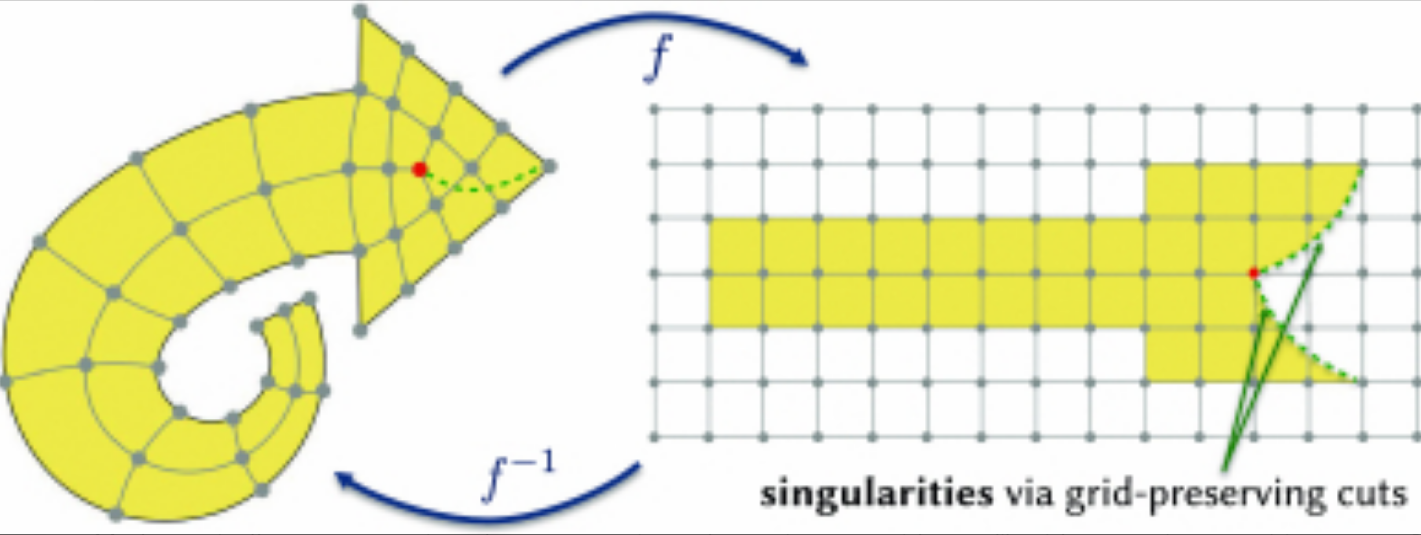
\includegraphics[width=30em]{figures/integer-grid-rough}
  \caption{Idea of quadrangulation with integer-grid maps in 2D (Figure from \cite{Hex22})}
  \label{fig:integer-grid}
\end{figure}
Directly searching for good Integer-Grid maps that minimize distortion and satisfy the boundary alignment
condition is a hard mixed-integer and non-convex optimization problem, for which no current
optimization technique is available that would result in an acceptable solution.

\subsection{Frame fields as a relaxation}
By taking the Jacobian of the seamless map, $\nabla \phi$, we get a mapping
$\nabla \phi : \mathcal{M} \to \mathbb{R}^{3\times3}$ of \emph{frames}, a \emph{frame field}.
The idea of frame fields is to then search for an approximation of $\nabla \phi$.
If $F: \mathcal{M} \to \mathbb{R}^{3\times3}$ is the approximation of $\nabla \phi$, we can
solve for $\phi : \mathcal{M} \to \mathbb{R}^3$ with
\begin{equation}\label{eq:poisson}
  \min \limits_{\phi} \int \limits_{\mathcal{M}} ||\nabla \phi F - \Id||^2
\end{equation}
where $||\cdot||$ is the Frobenius norm. If this is sufficiently small, then $F^{-1} \approx \nabla \phi$ and 
the extracted hexahedral mesh closely follow the integer isolines.
A frame locally represents the edges of a deformed cube.
We can think of a frame field as the composition of three vector fields
and as a relaxation of the original problem. However, frame fields
can contain singularities that the underlying vector fields do not contain \cite{Nieser}
and contain types of singularities that cannot appear in hex meshes \cite{Liu}.
These singularities are said to be non-meshable.
The problem of non-meshability is not discussed further here, but it
is something to be aware of.

We treat a frame $F$ as a set of 3 linearly independent vectors $\{F_1,F_2,F_3 \}$ which we can
collect into a matrix $F=(F_1,F_2,F_3) \in \mathbb{R}^{3\times 3}$.
Notice that many of these frames are equivalent.
There are $2^3$ choices of the sign, and $3!$ possible permutations, which
gives $2^3\cdot 3! = 48$ equivalent frames.
Since we want non-degenerate frames and the same orientation through the grid, the constraint $\det(F)>0$ is imposed,
which leaves $24$ equivalent frames.
Equivalence of frames is then defined as
$$F_u \sim F_v \iff \exists R \in \mathcal{O} : F_u=RF_v$$
where $\mathcal{O}$ is the \emph{chiral cubical symmetry group}\cite{Nieser}.
These symmetries complicate the optimization process for frame fields.
When optimizing the smoothness of a frame field, frames have to be compared.
To compare frames, we need to check if the vectors making up
the frames point in the same direction or if they have to be rotated
by some matrix $M \in \mathrm{SO}(3)$ first, to make them point in the same direction.
But now, the mentioned symmetry of representing the frames in $\mathbb{R}^3$
make $M$ ambiguous (${M_1 = RM_2, R \in \mathcal{O}}$).
Therefore, we instead use the spherical harmonics based representation to represent frames \cite{Huang}.
The idea is to represent frames as rotations of the polynomial $\mathbb{P}=x^4+y^4+z^4$,
and these rotations of the polynomial are naturally invariant under $\mathcal{O}$.
Under the restriction of the 4th degree polynomials to the sphere, that is $\mathbb{S}^2\to \mathbb{R}$,
the polynomials form a 9D vector space and the spherical harmonics of the 4th band form a basis.
For example, the axis-aligned frame $F=(e_1,e_2,e_3)$ corresponds
to $\mathbb{P}$, as $\mathbb{P}$ under the restriction to the sphere takes its maxima at $\pm e_i$.


The action of rotating 4th degree polynomials can be represented by so called $9\times9$ \emph{Wigner D-matrices}.
These Wigner D-matrices and rotation matrices in $\mathbb{R}^3$ both represent the
same elements of the group $\mathrm{SO}(3)$, just act on different vector spaces.
It is clear that this is a relaxation: Since rotations in 3D only exhibit 3 degrees of freedom, not all 9D spherical harmonic vectors are valid rotations
of $x^4+y^4+z^4$.

While optimizing the frame field, some kind of ``average'' of two frames will be done.
This averaging makes sense in the spherical harmonics space, but the result may be outside the valid
space of frames. A projection from the spherical
harmonics space back to the valid space of frames will be needed, see figure \ref{fig:projection} \cite{Ray}.
\begin{figure}[htb]
  \centering
  \def\svgwidth{30em}
  \input{figures/projection.pdf_tex}
  \caption{Combination of two valid frames leads to a resulting frame outside the valid frames. A projection to the nearest valid frame is done.}
  \label{fig:projection}
\end{figure}


When a frame $F$ has orthonormal columns, the resulting hex elements resemble unit cubes.
By introducing a metric $g$, we can control the size and shear of the cubes by
relaxing the orthonormality constraint to $g$-orthonormality when
$F^{-1}gF = \Id$
holds. We can decompose the frame field $F$ into a rotational part $R : \mathcal{M} \to \text{SO}(3)$ and a symmetric metric part $g^{-1/2}$
(akin to the polar decomposition of linear transformations)\cite{Panozzo}, that is $F = g^{-1/2}R$,
see figure \ref{fig:factorization}.
\begin{figure}[htb]
  \centering
  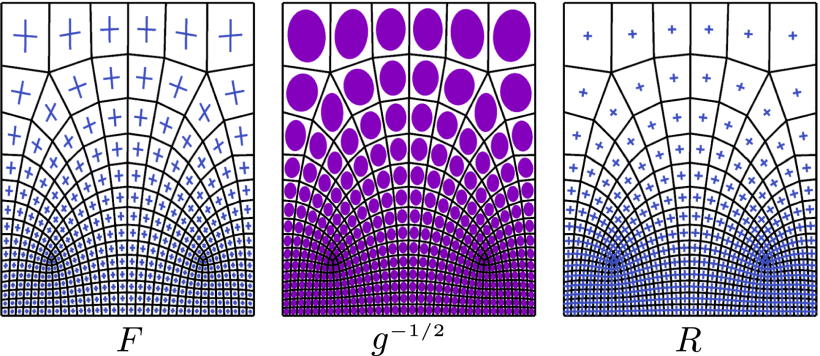
\includegraphics[width=25em]{figures/factorization}
  \caption{Factorization of a $g$-orthogonal frame field into a symmetric metric part $g^{-1/2}$ and a rotational part $R$
  (Figure from \cite{Fang23}).}
  \label{fig:factorization}
\end{figure}
Requirements for a frame field are usually formulated as
\begin{itemize}
  \item Smoothness: by minimizing the Dirichlet energy $E(F)=\int_{\mathcal{M}}||\nabla F||^2 dV $, the smoothness within the frame field is maximized which minimizes distortion of the seamless map;
  \item Boundary alignment: one of the columns of the frame field should match with the surface normal such that the hex elements accurately trace the surface of the object;
  \item Integrability: to find $\phi$ with equation \ref{eq:poisson}, the frame field must be as close to integrable as possible.
\end{itemize}

\end{document}